\chapter{Additional Case Studies}

\label{chapter_additional_case_studies}

\section{Application to Shallow Water Waves}
\label{sec_ocean_wave}

\subsection{Setup}
Our first additional case study is an exemplary hydrodynamics problem constructed to demonstrate an application to the analysis of water waves.  The problem setup is as follows.  A traveling water wave modeled by the classic soliton solution (\ref{eq_solitonkdv}) to the well-known Korteweg-De Vries (KdV) equation which passes an ocean buoy at time $t=0$ and position $x=0$ along a horizontal axis $x$.  The buoy measures the wavenumber $k$ with some error $\varepsilon$ such that the true wavenumber falls within a range $k \in \left[k_a, k_b\right]$ where $k_a = k-\varepsilon$ and $k_b = k+\varepsilon$ such that the height at a given horizontal position $x$ and time $t$ is given by
\begin{align}
	\label{eq_solitonkdv}
	\eta(x, t, k) = 12 k^2 \sech^2(kx-4k^3t) .
\end{align}
Assuming that the true wavenumber $k$ can fall anywhere in $\left[k_a, k_b\right]$ with equal probability we desire to know the mean wave height $\bar{\eta}(t_c, x_c, k)$ given by \eqref{eq_meanwave} at some constant time $t_c$ at another buoy at constant horizontal location $x_c$:
\begin{align}
	\label{eq_meanwave}
	\bar{\eta}(x_c, t_c, k) = 
	\frac{12}{k_b - k_a}
	\int_{k_a}^{k_b} \! 
	k^2 \sech^2(k x_c - 4 k^3 t_c) \,
	\mathrm{d}k.
\end{align}
\begin{figure}[!htb]
	
\includegraphics[width=\textwidth]{images/NonlinearWave.png}
	\caption[Nonlinear Wave]{\label{fig_nonlinear_wave} Nonlinear wave.}
\end{figure}


The integral of \eqref{eq_meanwave} is resistant to analytical solutions.  Although it can be solved via numerical methods we desire an analytical solution to serve as a standard which various available numerical methods can be evaluated against and independently checked.  To this end, an attempt can be made to arrive at an analytically tractable form by a Taylor series expansion of $\sech^2(v)$.  However, this is only valid within the convergent region of the Taylor series, i.e., $|kx_c - 4k^3t_c| < \frac{\pi}{2}$ and even mild choices of the parameters $k$, $x_c$, and $t_c$ exceed these bounds.  We therefore require an expansion that can be employed to arrive at an analytical form valid for a desired range of arguments $|kx_c - 4k^3t_c| < V$.  Furthermore, since we intend to use this expansion as a means by which numerical calculations are checked independently, we also require exact coefficients, exact error formulas, and therefore require an expansion with the properties highlighted in Table \ref{table_qualitative_comparison}.

\subsection{Solution}
We seek to know the mean wave height $\bar{\eta}(x_c, t_c, k)$ given the uncertainty about the
wavenumber $k$ at the critical range $x_c$ and the critical time $t_c$.  We begin by recalling
from Chapter \ref{chapter_improved_expansions} that $\sech^2(v) = \sum_{m=0}^{M} U_{2m}(M) v^{2m}$
and employing the expansion to break up the integral of Eq. \ref{eq_meanwave} via
\begin{align}
	\bar{\eta}(x_c, t_c, k)
	    &= \frac{12}{k_b - k_a}
	    \int_{k_a}^{k_b} \! 
	    k^2 \sech^2(k x_c - 4 k^3 t_c) \,
	    \mathrm{d}k \nonumber\\
	    &\simeq \frac{12}{k_b - k_a} \sum_{m=0}^{M} U_{2m}(M)
	        \int_{k_a}^{k_b} \! k^2 (k x_c - 4 k^3 t_c)^{2m} \, \mathrm{d}k.
\end{align}
Integrating directly yields
\begin{align}
	\Lambda(k) &= \int \! k^2 (k x_c - 4 k^3 t_c)^{2m} \, \mathrm{d}k \nonumber \\
	    &= \frac{k^3}{2m+3}\left( \frac{k x_c - 4 k^3 t_c}{1 - \frac{4 k^2 t_c}{x_c}} \right)^{2m}
	      \, _2F_1\left(-2m,\frac{2m+3}{2};\frac{2m+5}{2}; \frac{4 k^2 t_c}{x_c}\right)
\end{align}
such that the mean wave height can be expressed as
\begin{align}
	\bar{\eta}(x_c, t_c, k)
	&= \frac{12}{k_b - k_a} \sum_{m=0}^{M} U_{2m}(M)\left(\Lambda(k_b) - \Lambda(k_a)\right).
\end{align}

\subsection{Results}
Figs. \ref{fig_sech2_tc_sweep} and \ref{fig_sech2_xc_sweep} show the
mean wave height $\bar{\eta}(x_c, t_c, k)$ as $t_c$ and $x_c$ are
varied respectively.  The agreement of the numerical and analytical methods
indicates that a reliable method of analyzing the wave height for uncertain
wavenumber has been achieved.  Data was collected for a wave with
uniformly distributed $k \in [0.9, 1.2]$.  For the expansions employed in the
analytical results $M = 50$ terms were used with a range of validity $V = 10$.
For the integrals employed in the numerical results a step of $\Delta t = 0.0001$
was used.
\begin{figure}[!htp]
	\centering
	\textit{Mean wave height for $k \in [0.9, 1.2]$ at $x_c = 5$}\par
	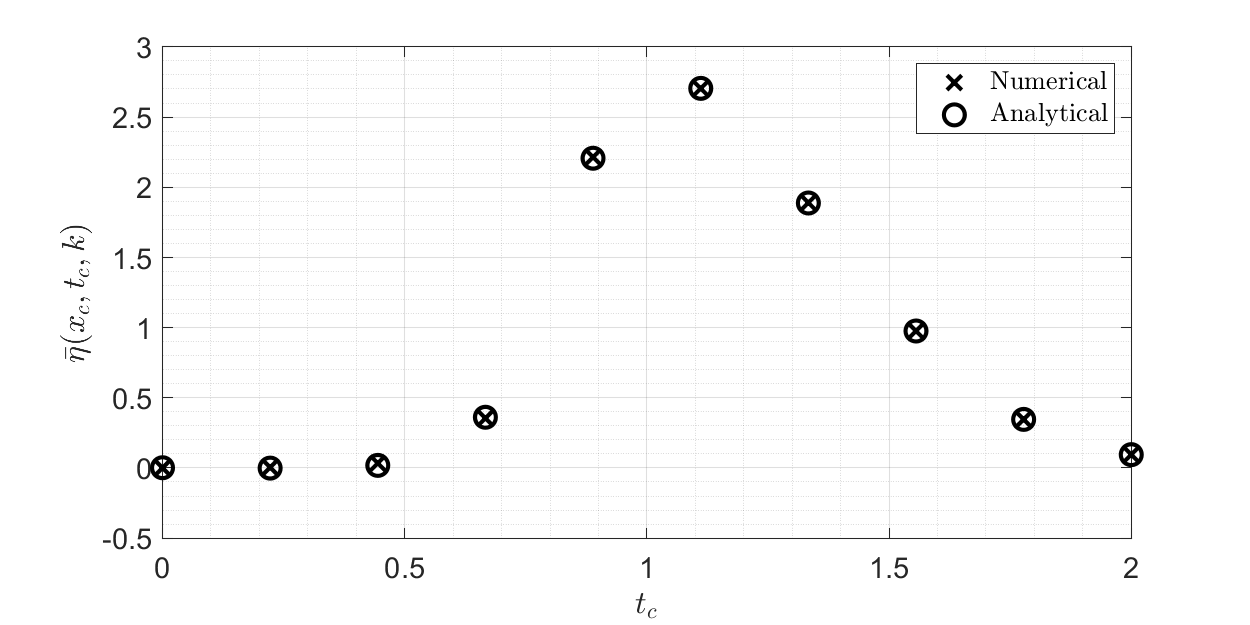
\includegraphics[width=0.9\textwidth]{Images/tc_sweep.png}
	\caption[Mean Wave Height with Respect to Time]{Mean wave height at $x_c$ with respect to $t_c$.}
	\label{fig_sech2_tc_sweep}
\end{figure}
\begin{figure}[!hbp]
	\centering
	\textit{Mean wave height for $k \in [0.9, 1.2]$ at $t_c = 1$}\par
	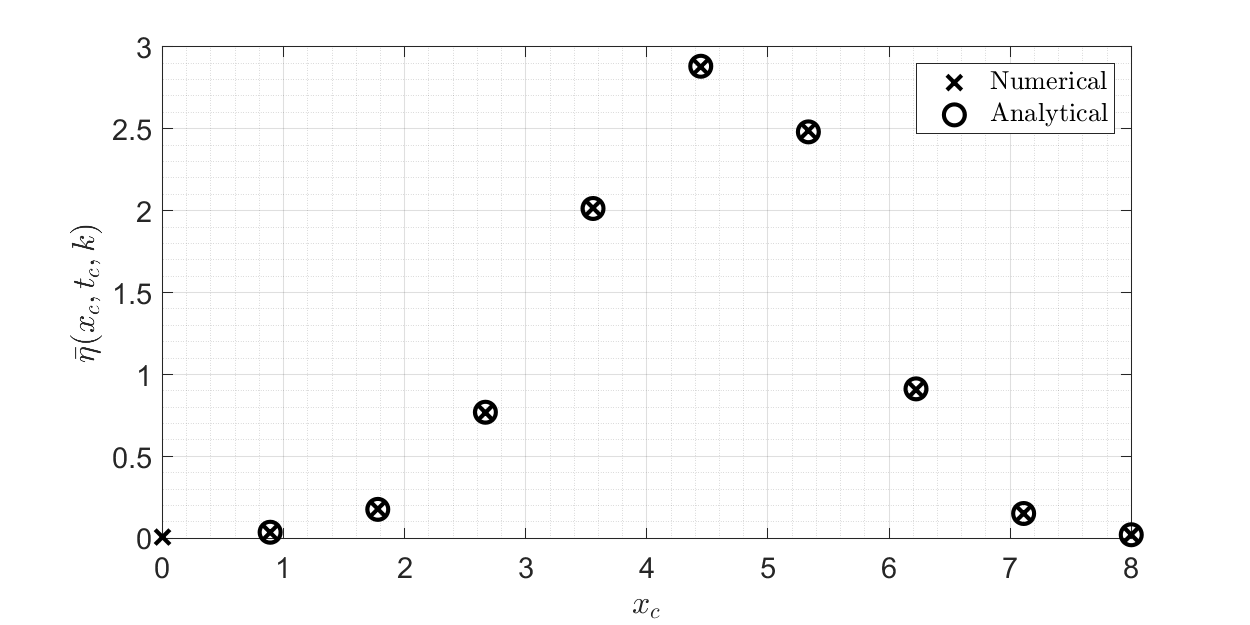
\includegraphics[width=0.9\textwidth]{Images/xc_sweep.png}
	\caption[Mean Wave Height with Respect to Position]{Mean wave height at $t_c$ with respect to $x_c$.}
	\label{fig_sech2_xc_sweep}
\end{figure}


\section{Application to Nonlinear Circuit Analysis}

\label{sec_nonlinear_amplifier}

\subsection{Setup}
Our second additional case study is drawn from practical problems in nonlinear circuit analysis.  The problem setup is as follows.  A nonlinear amplifier represented by a simplified hyperbolic tangent model such as that used in \cite{abdelfattah_modeling_2006} is stimulated by an input $x(t)$ to produce an output $y(t)$:
\begin{align}
	y(t) = \tanh(g x(t) + d).
\end{align}
We consider both unbiased and biased amplifiers.  The input is set to $x(t) = \sin(\omega t)$ and we desire to know the strength of the Fourier harmonics with respect to the gain $g$ and the D.C. bias $d$:
\begin{align}
	a_0(g, d) &= \frac{\omega}{\pi}
	\int_{0}^{\frac{2 \pi}{\omega}} \! 
	\tanh(g \sin(\omega t) + d) \,
	\mathrm{d}t , \label{eq_fourier_a0_integral} \\
	a_n(g, d) &= \frac{\omega}{\pi}
	\int_{0}^{\frac{2 \pi}{\omega}} \! 
	\tanh(g \sin(\omega t) + d) \cos(n \omega t) \,
	\mathrm{d}t , \label{eq_fourier_an_integral} \\
	b_n(g, d) &= \frac{\omega}{\pi}
	\int_{0}^{\frac{2 \pi}{\omega}} \! 
	\tanh(g \sin(\omega t) + d) \sin(n \omega t) \,
	\mathrm{d}t . \label{eq_fourier_bn_integral}
\end{align}

\begin{figure}[!htb]
	
\includegraphics[width=\textwidth]{images/NonlinearAmplifier.png}
	\caption[Nonlinear Amplifier without Input Bias]{\label{nl_amp_without_bias} Nonlinear amplifier without input bias.}
	\label{fig_nl_amp_no_bias}
\end{figure}

\begin{figure}[!htb]
	
\includegraphics[width=\textwidth]{images/NonlinearAmplifierWithBias.png}
	\caption[Nonlinear Amplifier with Input Bias]{\label{nl_amp_with_bias} Nonlinear amplifier with input bias.}
    \label{fig_nl_amp_with_bias}
\end{figure}

Again, the integrals in (\ref{eq_fourier_a0_integral}-\ref{eq_fourier_bn_integral}) are resistant to analytical solutions.  For an unbiased excitation (i.e., $d=0$) the $a_n$ coefficients are equal to $0$.  However, the integrals for $b_n$ are still non-trivial, and we find them resistant to direct solution even by powerful computer algebra systems. As with the example of \ref{sec_ocean_wave}, the integrals can easily be solved numerically, however we desire an analytical solution to serve as a standard which various numerical methods can be evaluated against to identify solutions which optimize the trade-off between accuracy and computational efficiency for a given application.  We seek agreement between analytical and numerical methods as indication that both solutions are correct and neither is rendered unreliable by unaccounted errors.  Furthermore, we desire analytical forms for the results which can be further manipulated and analyzed to extract useful patterns and make informed design decisions.

The Taylor series of the $\tanh(v)$ facilitates analysis of small signals where $\mathrm{max}(|g\sin(\omega t) + d|) < \frac{\pi}{2}$ but does not permit analysis of strong nonlinearity.  As noted for analysis of the $\tanh$ in neural networks, other well-known approximations such as $\tanh(v) = 1 + 2 \sum_{m=1}^{\infty}(-1)^m e^{-2mv} \ \forall \  v > 0$ permit analysis of large signals but not small signals.  We require here an analytical form valid for a desired range of arguments $\mathrm{max}(|g\sin(\omega t) + d|) < V$.  Again, since we intend to use this expansion as a means by which numerical calculations are checked independently, we also require exact coefficients, exact error formulas, and therefore require an expansion with the properties highlighted in Table \ref{table_qualitative_comparison}.  The utility of the AMITE technique
to this end is demonstrated in two example problems considering amplifiers with and without input D.C. bias.  In both problems the exact solutions
to the integrals therein yield novel integer sequences
which have never before been registered with the Online Encyclopedia of Integer Sequences (OEIS).
These sequences have since been submitted to the OEIS as part of the contribution this thesis
makes to the academic community.

\subsection[Problem 1: Unbiased Nonlinear Amplifier]{Problem 1: Unbiased Nonlinear Amplifier}

In this problem we consider the unbiased amplifier of Fig. \ref{fig_nl_amp_no_bias}.
We desire to know the strength of the output harmonics $b_n$ with respect to the
input gain $g$.  Therefore, we consider the integral
\begin{align}
	b_n (g) = \int_{-\pi}^{\pi} \! \tanh(g \sin(t)) \sin(nt) \, \mathrm{d}t.
\end{align}
We treat this integral with the AMITE technique and extract a solution in terms a novel integer
sequence.  The derivation of the sequence and a method of generating its entries is
provided.

\subsubsection{Solution}
We begin with the expression for the output harmonics, noting that for unbiased
excitation only the $b_n(g)$ terms are present in the output.
Recalling from Chapter \ref{chapter_improved_expansions} that
$\tanh(v) \simeq \sum_{m=0}^{M} T_{2m+1}(M) v^{2m+1}$,
we break up the integral for $b_n(g)$ via the AMITE polynomials yielding
\begin{align}
	b_n(g) &= \frac{1}{\pi}\int_{-\pi}^{\pi} \! \tanh(g \sin(t)) \sin(nt) \, \mathrm{d}t \\
	       &\simeq \frac{1}{\pi} \sum_{m=0}^{M} T_{2m+1}(M) g^{2m+1}
	                            \int_{-\pi}^{\pi} \sin^{2m+1}(t) \sin(nt) \, \mathrm{d}t.
	                            \label{eq_nl_gain_integral}
\end{align}
Noting that the result is a trigonometric polynomial, we desire a method
for generating the coefficients thereof exactly in the general case
without having to expand the integrand manually.  We achieve this by
attacking the integral directly via
\begin{align}
	&\int \sin^{2m+1}(t) \sin(nt) \, \mathrm{d}t \nonumber\\
	&\quad\quad= -\frac{i 4^{-m-1} \left(1-e^{2 i t}\right)^{-2 m} \left(-i e^{-i t}
		\left(-1+e^{2 i t}\right)\right)^{2 m} e^{-i (n+1) t}
		    \left(
                q h_1(t) - r e^{2 i n t} h_2(t)
            \right)}{q r}.
\end{align}
Here the sub-expressions are given:
\begin{align*}
	q &= 2 m-n+1, \\
	r &= 2 m+n+1, \\
	h_1(t) &= \, _2F_1\left(-2 m-1,-m-\frac{n}{2}-\frac{1}{2};-m-\frac{n}{2}+\frac{1}{2};e^{2 i t}\right), \\
	h_2(t) &= \, _2F_1\left(-2 m-1,\frac{1}{2} (-2 m+n-1);\frac{1}{2} (-2 m+n+1);e^{2 i t}\right).
\end{align*}
Simplifying reveals the occurrence of the Euler Beta function
\begin{align}
	&\int \sin^{2m+1}(t) \sin(nt) \, \mathrm{d}t = \nonumber\\
	&\quad\quad\frac{i}{8} \left(1-e^{2 i t}\right)^{-2 m}
	    e^{-i (n+1) t} \sin ^{2 m}(t)
	    \left(
	        \left(e^{2 i t}\right)^{\frac{r}{2}}
	            \mathrm{B}_{e^{2 i t}}\left(-\frac{r}{2},2 m+2\right)
	            +\frac{2 e^{2 i n t} h_2(t)}{q}\right).
\end{align}
Noting symmetry of the integrand, the definite integral must be evaluated
from $t = 0$ to $t = \pi$. This reveals the expression
\begin{align}
	&\int_{0}^{\pi} \sin^{2m+1}(t) \sin(nt) \, \mathrm{d}t \nonumber\\
	&\quad\quad = \frac{i \pi  2^{-2 m-3} e^{-i \pi  n} \left(1+e^{i \pi  n}\right) \Gamma (2 m+2) \left(\sec \left(\frac{1}{2} \pi  (2 m+n)\right)-e^{i \pi  n} \sec \left(\pi  m-\frac{\pi  n}{2}\right)\right)}{\Gamma \left(m-\frac{n}{2}+\frac{3}{2}\right) \Gamma \left(m+\frac{n}{2}+\frac{3}{2}\right)}.
\end{align}
The expression is undefined for $n \in \mathbb{W}$ but has well defined limits
which can be used to extract the exact values of the integral which can then
be substituted back into Eq. (\ref{eq_nl_gain_integral})
to evaluate the coefficients of the expansion precisely.
Taking the limit as $n$ approaches whole numbers allows conveniently generating
the exact values of the integral, i.e.,
\begin{align}
	&\mu_{n', m} =\nonumber\\
	&\ \ \lim_{n \to n'}
	\frac{i \pi  2^{-2 m-3} e^{-i \pi  n} \left(1+e^{i \pi  n}\right) \Gamma (2 m+2) \left(\sec \left(\frac{1}{2} \pi  (2 m+n)\right)-e^{i \pi  n} \sec \left(\pi  m-\frac{\pi  n}{2}\right)\right)}{\Gamma \left(m-\frac{n}{2}+\frac{3}{2}\right) \Gamma \left(m+\frac{n}{2}+\frac{3}{2}\right)}, \\
	&\quad\quad\forall\quad n' \in \mathbb{W},\ m \in \mathbb{W}. \nonumber
\end{align}
The results are tabulated in Table \ref{table_unbiased_sequences}.  The numerators comprise a family
of novel integer sequences not present in the OEIS.

\begin{table}
\caption{$\mu_{n,m} \ \forall \ n \in [0,7], m \in [0,20]$ }
\label{table_unbiased_sequences}
\begin{tabular}{|L||L|L|L|L|L|L|L|L|}
\hline
& \multicolumn{8}{|c|}{$n$} \\
\hline
m & 0 & 1  & 2 & 3 & 4 & 5 & 6 & 7 \\
\hline
\hline
0 & 0 & \pi  & 0 & 0 & 0 & 0 & 0 & 0 \\
1 & 0 & -\frac{3 \pi }{4} & 0 & \frac{\pi }{4} & 0 & 0 & 0 & 0 \\
2 & 0 & \frac{5 \pi }{8} & 0 & -\frac{5 \pi }{16} & 0 & \frac{\pi }{16} & 0 & 0 \\
3 & 0 & -\frac{35 \pi }{64} & 0 & \frac{21 \pi }{64} & 0 & -\frac{7 \pi }{64} & 0 & \frac{\pi }{64} \\
4 & 0 & \frac{63 \pi }{128} & 0 & -\frac{21 \pi }{64} & 0 & \frac{9 \pi }{64} & 0 & -\frac{9 \pi }{256} \\
5 & 0 & -\frac{231 \pi }{512} & 0 & \frac{165 \pi }{512} & 0 & -\frac{165 \pi }{1024} & 0 & \frac{55 \pi }{1024} \\
6 & 0 & \frac{429 \pi }{1024} & 0 & -\frac{1287 \pi }{4096} & 0 & \frac{715 \pi }{4096} & 0 & -\frac{143 \pi }{2048} \\
7 & 0 & -\frac{6435 \pi }{16384} & 0 & \frac{5005 \pi }{16384} & 0 & -\frac{3003 \pi }{16384} & 0 & \frac{1365 \pi }{16384} \\
8 & 0 & \frac{12155 \pi }{32768} & 0 & -\frac{2431 \pi }{8192} & 0 & \frac{1547 \pi }{8192} & 0 & -\frac{1547 \pi }{16384} \\
9 & 0 & -\frac{46189 \pi }{131072} & 0 & \frac{37791 \pi }{131072} & 0 & -\frac{12597 \pi }{65536} & 0 & \frac{6783 \pi }{65536} \\
10 & 0 & \frac{88179 \pi }{262144} & 0 & -\frac{146965 \pi }{524288} & 0 & \frac{101745 \pi }{524288} & 0 & -\frac{14535 \pi }{131072} \\
11 & 0 & -\frac{676039 \pi }{2097152} & 0 & \frac{572033 \pi }{2097152} & 0 & -\frac{408595 \pi }{2097152} & 0 & \frac{245157 \pi }{2097152} \\
12 & 0 & \frac{1300075 \pi }{4194304} & 0 & -\frac{557175 \pi }{2097152} & 0 & \frac{408595 \pi }{2097152} & 0 & -\frac{2042975 \pi }{16777216} \\
13 & 0 & -\frac{5014575 \pi }{16777216} & 0 & \frac{4345965 \pi }{16777216} & 0 & -\frac{13037895 \pi }{67108864} & 0 & \frac{8436285 \pi }{67108864} \\
14 & 0 & \frac{9694845 \pi }{33554432} & 0 & -\frac{67863915 \pi }{268435456} & 0 & \frac{51895935 \pi }{268435456} & 0 & -\frac{17298645 \pi }{134217728} \\
15 & 0 & -\frac{300540195 \pi }{1073741824} & 0 & \frac{265182525 \pi }{1073741824} & 0 & -\frac{206253075 \pi }{1073741824} & 0 & \frac{141120525 \pi }{1073741824} \\
16 & 0 & \frac{583401555 \pi }{2147483648} & 0 & -\frac{64822395 \pi }{268435456} & 0 & \frac{51175575 \pi }{268435456} & 0 & -\frac{71645805 \pi }{536870912} \\
17 & 0 & -\frac{2268783825 \pi }{8589934592} & 0 & \frac{2029964475 \pi }{8589934592} & 0 & -\frac{405992895 \pi }{2147483648} & 0 & \frac{289994925 \pi }{2147483648} \\
18 & 0 & \frac{4418157975 \pi }{17179869184} & 0 & -\frac{7952684355 \pi }{34359738368} & 0 & \frac{6437887335 \pi }{34359738368} & 0 & -\frac{585262485 \pi }{4294967296} \\
19 & 0 & -\frac{34461632205 \pi }{137438953472} & 0 & \frac{31179571995 \pi }{137438953472} & 0 & -\frac{25510558905 \pi }{137438953472} & 0 & \frac{18855630495 \pi }{137438953472} \\
20 & 0 & \frac{67282234305 \pi }{274877906944} & 0 & -\frac{30582833775 \pi }{137438953472} & 0 & \frac{25264080075 \pi }{137438953472} & 0 & -\frac{75792240225 \pi }{549755813888} \\
\hline
\end{tabular}
\end{table}

\subsubsection{Results}
Figs. \ref{fig_harmonic1}, \ref{fig_harmonic3}, and \ref{fig_harmonic5}, show the
increase of the first, third, and fifth output harmonics with respect to the gain
of the unbiased input signal.  Both numerical results and analytical results using the
method detailed above are shown.  The agreement of the numerical and analytical methods
indicates that a reliable method of analyzing the effect of input gain
on output harmonics has been achieved.  Data was collected from input gains ranging from
$g=0$ to $g=4$.  For the expansions employed in the analytical results $M = 30$ terms were 
used.  For the integrals employed in the numerical results a step of $\Delta t = 0.001$ was
used.  
\begin{figure}[!htp]
	\centering
	\textit{Output Harmonic $b_1(g)$}\par
	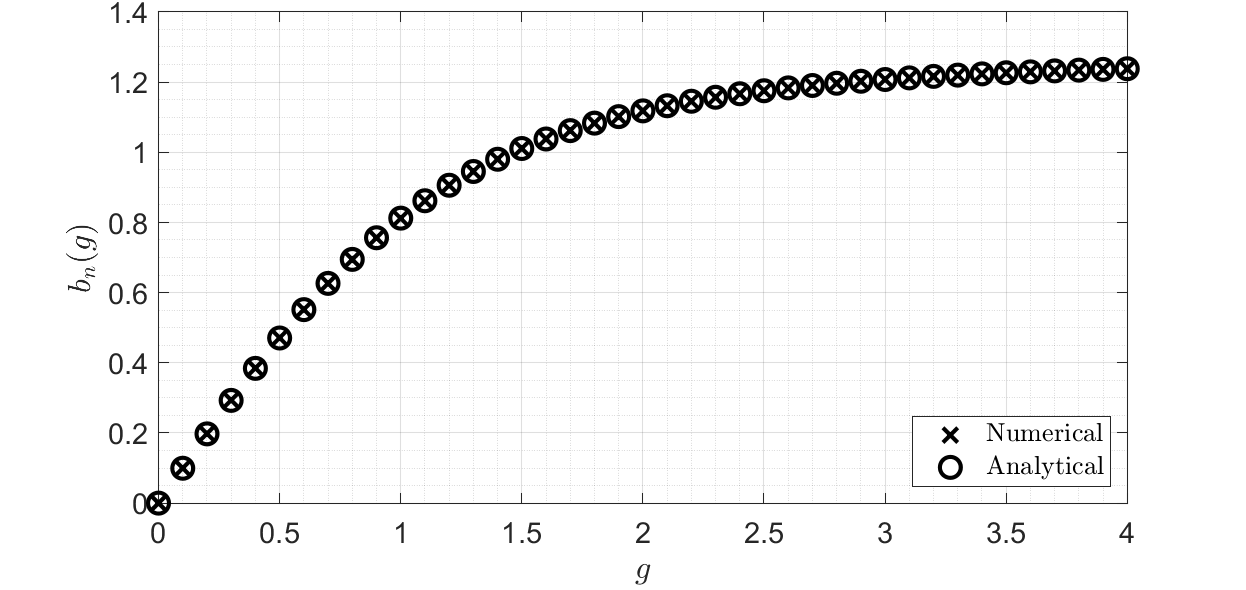
\includegraphics[width=0.6\textwidth]{Images/harmonic1.png}
	\caption[Harmonic $b_1(g)$]{Strength of output signal harmonic $b_1(g)$ with respect to input gain $g$.}
	\label{fig_harmonic1}
\end{figure}
\begin{figure}[!hbp]
	\centering
	\textit{Output Harmonic $b_3(g)$}\par
	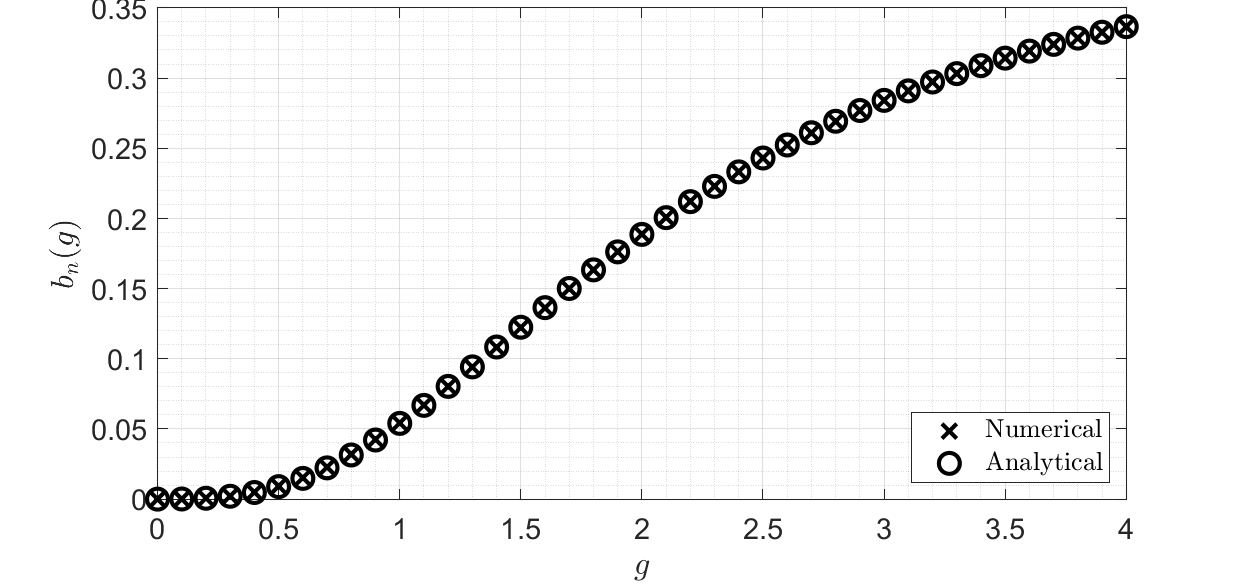
\includegraphics[width=0.6\textwidth]{Images/harmonic3.png}
	\caption[Harmonic $b_3(g)$]{Strength of output signal harmonic $b_3(g)$ with respect to input gain $g$.}
	\label{fig_harmonic3}
\end{figure}
\begin{figure}[!hbp]
	\centering
	\textit{Output Harmonic $b_5(g)$}\par
	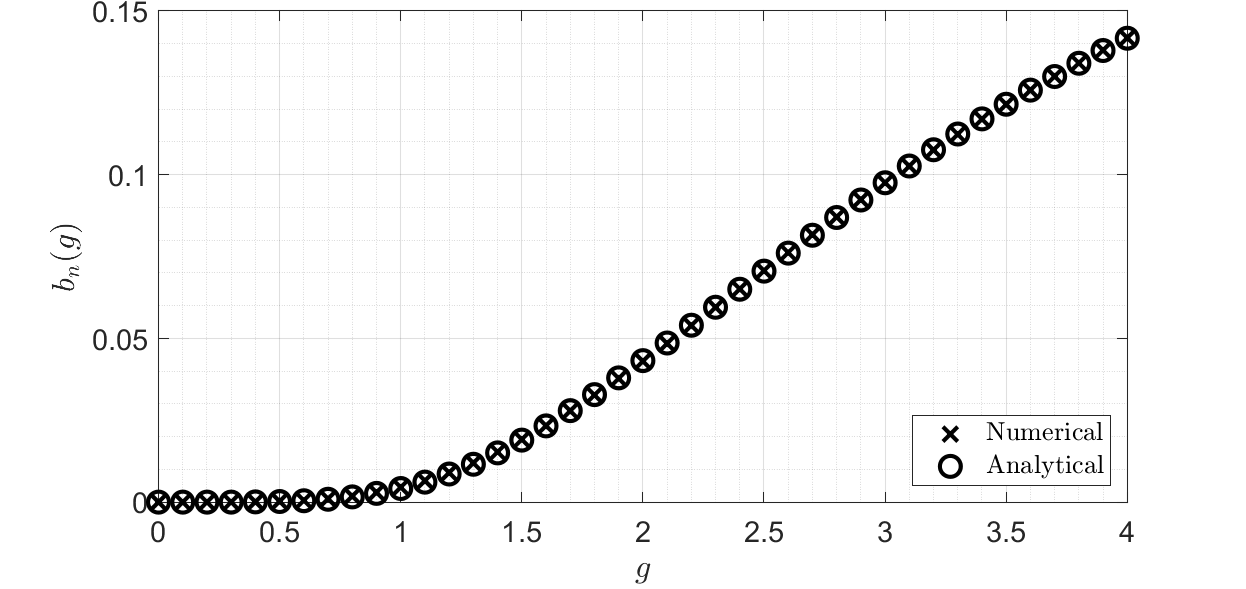
\includegraphics[width=0.6\textwidth]{Images/harmonic5.png}
	\caption[Harmonic $b_5(g)$]{Strength of output signal harmonic $b_5(g)$ with respect to input gain $g$.}
	\label{fig_harmonic5}
\end{figure}


\subsection{Problem 2: Output Bias of a Nonlinear Amplifier}

In this problem we consider the biased amplifier of Fig. \ref{fig_nl_amp_with_bias}.
We desire to know the relationship between the D.C. bias $a_0$ of the signal at output
and the D.C. bias, $d$, of the input giving full consideration to the mixing effects
due to the coupling of contributions the input gain, $g$, and input D.C. bias, $d$,
make to the output.  We therefore consider the integral
\begin{align}
	a_0(g, d) = \int_{0}^{2 \pi} \! \tanh(g \sin(t) + d) \, \mathrm{d}t.
\end{align}
We treat this integral with the AMITE technique to obtain the exact relationships
governing the mixing of the contributions of input gain and input D.C. bias to the
output.  The solution employed results in a function which generates several
novel integer sequences.  Their derivation is provided along with a method of
generating their entries.  Several embodiments of the general pattern are
tabulated and cataloged for convenience.

\subsubsection{Solution}
We begin with the expression for the output bias $a_0$.
As with the unbiased amplifier above, we recall from Chapter
\ref{chapter_improved_expansions} that
$\tanh(v) \simeq \sum_{m=0}^{M} T_{2m+1}(M) v^{2m+1}$.
We break up the integral for $a_0(g, d)$ via the AMITE polynomials yielding
\begin{align}
	a_0(g, d) &= \frac{1}{\pi}\int_{0}^{2\pi} \! \tanh(g \sin(t) + d) \, \mathrm{d}t \\
	&\simeq \frac{1}{\pi} \sum_{m=0}^{M} T_{2m+1}(M)
	\int_{0}^{2\pi} (g \sin(t) + d)^{2m+1} \, \mathrm{d}t.
	\label{eq_nl_gain_integral_a0}
\end{align}
As above, we note that the result is a trigonometric polynomial and desire a method
for generating the coefficients thereof exactly in the general case
without having to expand the integrand manually.  We achieve this by
attacking the integral directly via
\begin{align}
	\Lambda(t) &= \int (g \sin(t) + d)^{2m+1} \, \mathrm{d}t \\
	&=
	\frac{\sec (t) \sqrt{-\frac{g (\sin (t)-1)}{d+g}} \sqrt{\frac{g (\sin (t)+1)}{g-d}} (d+g \sin (t))^{2 m+2} h(t)}{2 g m+2 g}
\end{align}
where the sub-expression $h(t)$ is a short-hand for an Appell Hypergeometric Function:
\begin{align}
h(t) = F_1\left(2 m+2;\frac{1}{2},\frac{1}{2};2 m+3;\frac{d+g \sin (t)}{d-g},\frac{d+g \sin (t)}{d+g}\right).
\end{align}
Noting that the direct anti-derivative has discontinuities at
$t = \frac{\pi}{2}$ and $t = \frac{3\pi}{4}$ we define a
principal value by taking a one sided limit at the discontinuity
within the interval of integration.  Taking advantage of symmetry of the
integrand results in the definition
\begin{align}
	&\mathrm{P.V.} \int_0^{2\pi} \! (g \sin(t) + d)^{2m+1} \, \mathrm{d}t \nonumber \\
	&\quad\quad \triangleq 2 \, \mathrm P.V. \int_0^{\frac{\pi}{2}} (g \sin(t) + d)^{2m+1} \, \mathrm{d}t
	    + 2 \, \mathrm P.V. \int_{\pi}^{\frac{3\pi}{2}} (g \sin(t) + d)^{2m+1} \, \mathrm{d}t \\
	&\quad\quad \triangleq 2\left(\lim_{t\to{\frac{\pi}{2}}^{-}} \Lambda(t) - \Lambda(0)\right)
	    + 2\left(\lim_{t\to{\frac{3\pi}{2}}^{-}} \Lambda(t) - \Lambda(\pi)\right).
\end{align}
The individual limits evaluate to
\begin{align}
\lim_{t\to{\frac{\pi}{2}}^{-}} \Lambda(t) &= \frac{\sqrt{\pi } \sqrt{\frac{g}{g-d}} \sqrt{\frac{g}{d+g}} \Gamma (2 m+3) (d+g)^{2 m+2} \, _2F_1\left(\frac{1}{2},2 (m+1);2 m+\frac{5}{2};\frac{d+g}{d-g}\right)}{(2 g m+2 g) \Gamma \left(2 m+\frac{5}{2}\right)}, \\
\lim_{t\to{\frac{3\pi}{2}}^{-}} \Lambda(t) &= -\frac{\sqrt{\pi } \sqrt{-\frac{g}{d-g}} \sqrt{\frac{g}{d+g}} \Gamma (2 m+3) (d-g)^{2 m+2} \, _2F_1\left(\frac{1}{2},2 (m+1);2 m+\frac{5}{2};\frac{d-g}{d+g}\right)}{(2 g m+2 g) \Gamma \left(2 m+\frac{5}{2}\right)}.
\end{align}
The integral evaluates to
\begin{gather}
\begin{align}
	&\mathrm{P.V.} \int_0^{2\pi} \! (g \sin(t) + d)^{2m+1} \, \mathrm{d}t \nonumber \\
	&\quad\quad = -\frac{\sqrt{\pi } \sqrt{\frac{g}{g-d}} \sqrt{\frac{g}{d+g}} \Gamma (2 m+3) \left((d-g)^{2 m+2} h_1(t) - (d+g)^{2 m+2}h_2(t)\right)}{g (m+1) \Gamma \left(2 m+\frac{5}{2}\right)},
\end{align} \\
h_1(t) = {}_2F_1\left(\frac{1}{2},2 (m+1);2 m+\frac{5}{2};\frac{d-g}{d+g}\right), \\
h_2(t) = {}_2F_1\left(\frac{1}{2},2 (m+1);2 m+\frac{5}{2};\frac{d+g}{d-g}\right).
\end{gather}
As desired, this expression defines the exact relationship between the mixed contributions that the input
gain and input bias make to the output bias.  The expression is undefined for $g = d$ but has a well defined
limit at this point.  Therefore, the set of possible sequences, denoted $q_m(g, d)$ arising from this result
can be defined as
\begin{gather}
\begin{align}
	q_m(g,d)
	    = \lim_{g \to g'}
	        -\frac{\sqrt{\pi } \sqrt{\frac{g}{g-d}} \sqrt{\frac{g}{d+g}} \Gamma (2 m+3) \left((d-g)^{2 m+2} h_1(t) - (d+g)^{2 m+2}h_2(t)\right)}{g (m+1) \Gamma \left(2 m+\frac{5}{2}\right)}
\end{align} \\
    \forall \ d, g' \in \mathbb{Q},\ m \in \mathbb{W} \nonumber.
\end{gather}
The results for some rational values of $g$ and $d$ are tabulated in Tables
\ref{table_biased_sequences_g1}, \ref{table_biased_sequences_g2},
\ref{table_biased_sequences_d1}, \ref{table_biased_sequences_d2}.  The numerators of the
exact solutions in the table form a family of new integer sequences not present in the OEIS.

\begin{table}[!htp]
	\caption{$q_m(g, d) \ \forall \ m \in [0,10], d \in \{\frac{1}{4}, \frac{1}{2}, 1, 2\}, g=1$ }
	\label{table_biased_sequences_g1}
	\centering
	\begin{tabular}{|L||L|L|L|L|}
		\hline
		& \multicolumn{4}{|c|}{$d$} \\
		\hline
		m & \frac{1}{4} & \frac{1}{2} & 1 & 2 \\
		\hline
		\hline
		0 & \frac{\pi }{2} & \pi  & 2 \pi  & 4 \pi  \\
		1 & \frac{25 \pi }{32} & \frac{7 \pi }{4} & 5 \pi  & 22 \pi  \\
		2 & \frac{561 \pi }{512} & \frac{51 \pi }{16} & \frac{63 \pi }{4} & \frac{303 \pi }{2} \\
		3 & \frac{12489 \pi }{8192} & \frac{393 \pi }{64} & \frac{429 \pi }{8} & \frac{4587 \pi }{4} \\
		4 & \frac{281185 \pi }{131072} & \frac{3139 \pi }{256} & \frac{12155 \pi }{64} & \frac{290747 \pi }{32} \\
		5 & \frac{6418809 \pi }{2097152} & \frac{25653 \pi }{1024} & \frac{88179 \pi }{128} & \frac{4730157 \pi }{64} \\
		6 & \frac{148331665 \pi }{33554432} & \frac{212941 \pi }{4096} & \frac{1300075 \pi }{512} & \frac{156576859 \pi }{256} \\
		7 & \frac{3462260265 \pi }{536870912} & \frac{1787607 \pi }{16384} & \frac{9694845 \pi }{1024} & \frac{2623149099 \pi }{512} \\
		8 & \frac{81464917185 \pi }{8589934592} & \frac{15134931 \pi }{65536} & \frac{583401555 \pi }{16384} & \frac{354764780883 \pi }{8192} \\
		9 & \frac{1929237099225 \pi }{137438953472} & \frac{128996853 \pi }{262144} & \frac{4418157975 \pi }{32768} & \frac{6039703611897 \pi }{16384} \\
		10 & \frac{45928695279345 \pi }{2199023255552} & \frac{1105350729 \pi }{1048576} & \frac{67282234305 \pi }{131072} & \frac{206801268386001 \pi }{65536} \\
		\hline
	\end{tabular}
\end{table}

\begin{table}[!hbp]
	\caption{$q_m(g, d) \ \forall \ m \in [0,10], d \in \{\frac{1}{4}, \frac{1}{2}, 1, 2\}, g=2$ }
	\label{table_biased_sequences_g2}
	\centering
	\begin{tabular}{|L||L|L|L|L|}
		\hline
		& \multicolumn{4}{|c|}{$d$} \\
		\hline
		m & \frac{1}{4} & \frac{1}{2} & 1 & 2 \\
		\hline
		\hline
0 & \frac{\pi }{2} & \pi  & 2 \pi  & 4 \pi  \\
1 & \frac{97 \pi }{32} & \frac{25 \pi }{4} & 14 \pi  & 40 \pi  \\
2 & \frac{8001 \pi }{512} & \frac{561 \pi }{16} & 102 \pi  & 504 \pi  \\
3 & \frac{627873 \pi }{8192} & \frac{12489 \pi }{64} & 786 \pi  & 6864 \pi  \\
4 & \frac{48363649 \pi }{131072} & \frac{281185 \pi }{256} & 6278 \pi  & 97240 \pi  \\
5 & \frac{3701949153 \pi }{2097152} & \frac{6418809 \pi }{1024} & 51306 \pi  & 1410864 \pi  \\
6 & \frac{283146701761 \pi }{33554432} & \frac{148331665 \pi }{4096} & 425882 \pi  & 20801200 \pi  \\
7 & \frac{21695983405857 \pi }{536870912} & \frac{3462260265 \pi }{16384} & 3575214 \pi  & 310235040 \pi  \\
8 & \frac{1667338615773441 \pi }{8589934592} & \frac{81464917185 \pi }{65536} & 30269862 \pi  & 4667212440 \pi  \\
9 & \frac{128562758660255073 \pi }{137438953472} & \frac{1929237099225 \pi }{262144} & 257993706 \pi  & 70690527600 \pi  \\
10 & \frac{9946278255903268929 \pi }{2199023255552} & \frac{45928695279345 \pi }{1048576} & 2210701458 \pi  & 1076515748880 \pi  \\
		\hline
	\end{tabular}
\end{table}

\begin{table}[!htp]
	\caption{$q_m(g, d) \ \forall \ m \in [0,10], g \in \{\frac{1}{4}, \frac{1}{2}, 1, 2\}, d=1$ }
	\label{table_biased_sequences_d1}
	\centering
	\begin{tabular}{|L||L|L|L|L|}
		\hline
		& \multicolumn{4}{|c|}{$g$} \\
		\hline
		m & \frac{1}{4} & \frac{1}{2} & 1 & 2 \\
		\hline
		\hline
0 & 2 \pi  & 2 \pi  & 2 \pi  & 2 \pi  \\
1 & \frac{35 \pi }{16} & \frac{11 \pi }{4} & 5 \pi  & 14 \pi  \\
2 & \frac{2703 \pi }{1024} & \frac{303 \pi }{64} & \frac{63 \pi }{4} & 102 \pi  \\
3 & \frac{111939 \pi }{32768} & \frac{4587 \pi }{512} & \frac{429 \pi }{8} & 786 \pi  \\
4 & \frac{19428155 \pi }{4194304} & \frac{290747 \pi }{16384} & \frac{12155 \pi }{64} & 6278 \pi  \\
5 & \frac{869217429 \pi }{134217728} & \frac{4730157 \pi }{131072} & \frac{88179 \pi }{128} & 51306 \pi  \\
6 & \frac{79391968315 \pi }{8589934592} & \frac{156576859 \pi }{2097152} & \frac{1300075 \pi }{512} & 425882 \pi  \\
7 & \frac{3677961360195 \pi }{274877906944} & \frac{2623149099 \pi }{16777216} & \frac{9694845 \pi }{1024} & 3575214 \pi  \\
8 & \frac{1377344215036755 \pi }{70368744177664} & \frac{354764780883 \pi }{1073741824} & \frac{583401555 \pi }{16384} & 30269862 \pi  \\
9 & \frac{64983391570212225 \pi }{2251799813685248} & \frac{6039703611897 \pi }{8589934592} & \frac{4418157975 \pi }{32768} & 257993706 \pi  \\
10 & \frac{6169702305530824305 \pi }{144115188075855872} & \frac{206801268386001 \pi }{137438953472} & \frac{67282234305 \pi }{131072} & 2210701458 \pi  \\
		\hline
	\end{tabular}
\end{table}

\begin{table}[!hbp]
	\caption{$q_m(g, d) \ \forall \ m \in [0,10], g \in \{\frac{1}{4}, \frac{1}{2}, 1, 2\}, d=2$ }
	\label{table_biased_sequences_d2}
	\centering
	\begin{tabular}{|L||L|L|L|L|}
		\hline
		& \multicolumn{4}{|c|}{$g$} \\
		\hline
		m & \frac{1}{4} & \frac{1}{2} & 1 & 2 \\
		\hline
		\hline
0 & 4 \pi  & 4 \pi  & 4 \pi  & 4 \pi  \\
1 & \frac{131 \pi }{8} & \frac{35 \pi }{2} & 22 \pi  & 40 \pi  \\
2 & \frac{35343 \pi }{512} & \frac{2703 \pi }{32} & \frac{303 \pi }{2} & 504 \pi  \\
3 & \frac{4895907 \pi }{16384} & \frac{111939 \pi }{256} & \frac{4587 \pi }{4} & 6864 \pi  \\
4 & \frac{2776451387 \pi }{2097152} & \frac{19428155 \pi }{8192} & \frac{290747 \pi }{32} & 97240 \pi  \\
5 & \frac{401446357557 \pi }{67108864} & \frac{869217429 \pi }{65536} & \frac{4730157 \pi }{64} & 1410864 \pi  \\
6 & \frac{118001479249339 \pi }{4294967296} & \frac{79391968315 \pi }{1048576} & \frac{156576859 \pi }{256} & 20801200 \pi  \\
7 & \frac{17576234075546019 \pi }{137438953472} & \frac{3677961360195 \pi }{8388608} & \frac{2623149099 \pi }{512} & 310235040 \pi  \\
8 & \frac{21172707391056628563 \pi }{35184372088832} & \frac{1377344215036755 \pi }{536870912} & \frac{354764780883 \pi }{8192} & 4667212440 \pi  \\
9 & \frac{3216395485480034911137 \pi }{1125899906842624} & \frac{64983391570212225 \pi }{4294967296} & \frac{6039703611897 \pi }{16384} & 70690527600 \pi  \\
10 & \frac{984263326107473717711601 \pi }{72057594037927936} & \frac{6169702305530824305 \pi }{68719476736} & \frac{206801268386001 \pi }{65536} & 1076515748880 \pi  \\
		\hline
	\end{tabular}
\end{table}

\subsubsection{Results}
Figs. \ref{fig_output_bias_d_eq_1_2}, \ref{fig_output_bias_d_eq_1}, and \ref{fig_output_bias_d_eq_3_2}, show the
increase of the output D.C. bias with respect to the gain
of the input signal for D.C. input biases $d = \frac{1}{2}, 1, \frac{3}{2}$.
Both numerical results and analytical results using the
method detailed above are shown.  The agreement of the numerical and analytical methods
indicates that a reliable method of analyzing the effect of input gain
on output harmonics has been achieved.  Data was collected from input gains ranging from
$g=0$ to $g=4$.  For the expansions employed in the analytical results $M = 30$ terms were 
used.  For the integrals employed in the numerical results a step of $\Delta t = 0.001$ was
used.
\begin{figure}[!htp]
	\centering
	\textit{Output Bias for Input Bias $d = 1/2$}\par
	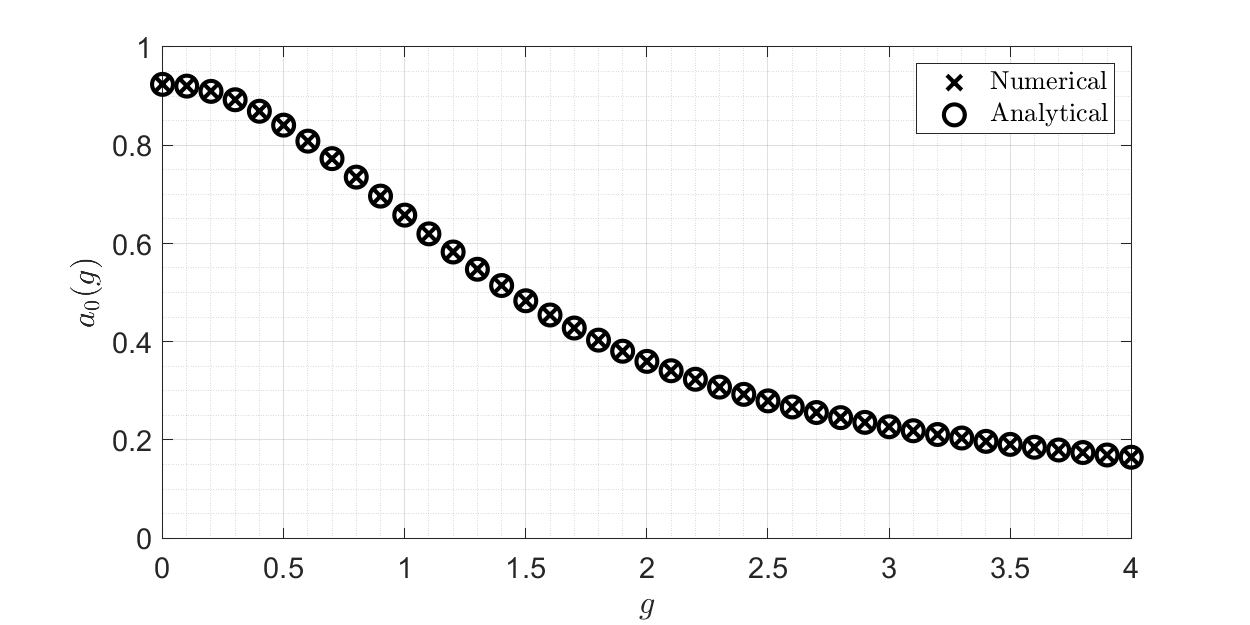
\includegraphics[width=0.6\textwidth]{Images/output_bias_for_input_bias_eq_0.50.png}
	\caption[Output Bias $a_0(g, d)$ for $d = 1/2$]{Output bias $a_0(g, d)$ with respect to input gain $g$ for input bias $d = 1/2$}
	\label{fig_output_bias_d_eq_1_2}
\end{figure}
\begin{figure}[!hbp]
	\centering
	\textit{Output Bias for Input Bias $d = 1$}\par
	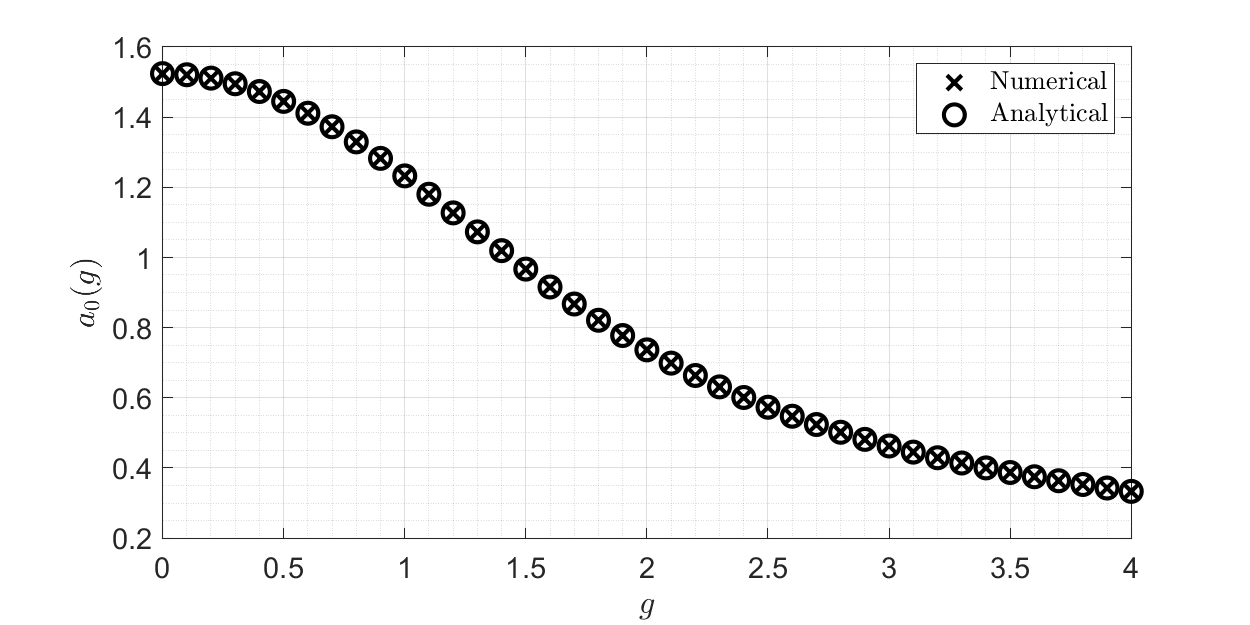
\includegraphics[width=0.6\textwidth]{Images/output_bias_for_input_bias_eq_1.00.png}
	\caption[Output Bias $a_0(g, d)$ for $d = 1$]{Output bias $a_0(g, d)$ with respect to input gain $g$ for input bias $d = 1$}
	\label{fig_output_bias_d_eq_1}
\end{figure}
\begin{figure}[!hbp]
	\centering
	\textit{Output Bias for Input Bias $d = 3/2$}\par
	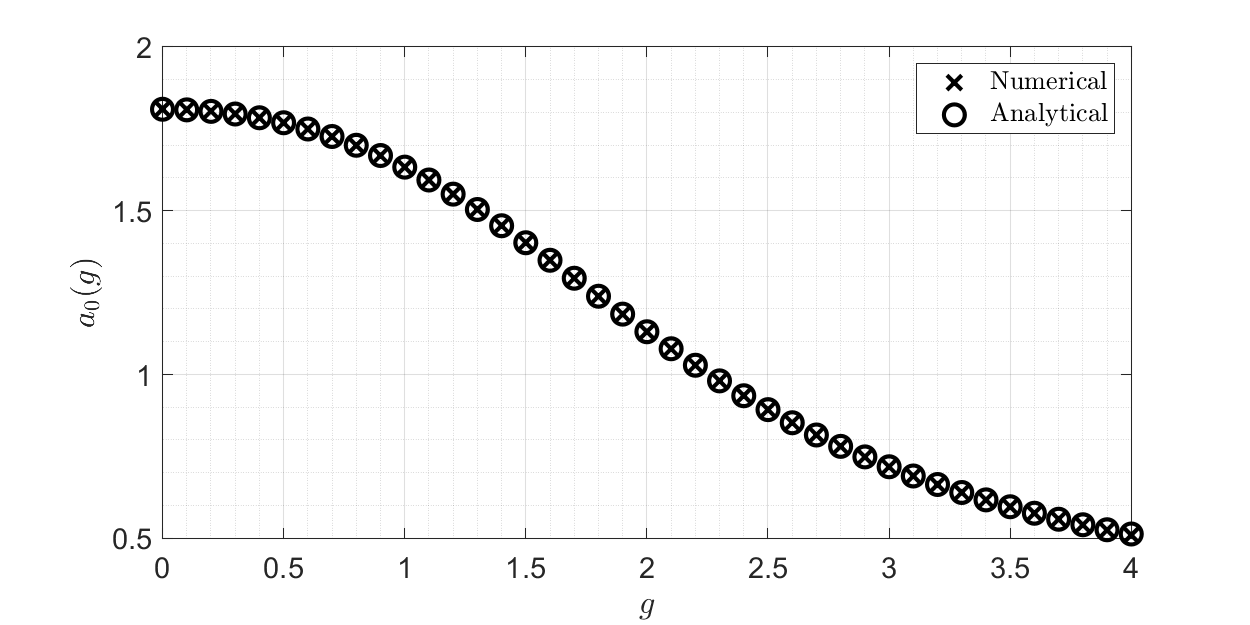
\includegraphics[width=0.6\textwidth]{Images/output_bias_for_input_bias_eq_1.50.png}
	\caption[Output Bias $a_0(g, d)$ for $d = 3/2$]{Output bias $a_0(g, d)$ with respect to input gain $g$ for input bias $d = 1$}
	\label{fig_output_bias_d_eq_3_2}
\end{figure}

